\documentclass[12pt,letterpaper]{article}
\usepackage[utf8]{inputenc}
\usepackage[T1]{fontenc}
\usepackage[spanish]{babel}
\usepackage{amsmath, amssymb}
\usepackage{geometry}
\usepackage{enumitem}
\usepackage{graphicx}

\geometry{margin=2.5cm}

\title{\textbf{Ejercicios tipo -- Certamen 3 -- Microeconomía I ICS-162}}
\date{}

\begin{document}

\maketitle

%=============================================================


%------------------------------------------------------------
\subsection*{Pregunta 1}

Amanda afirma que su situación como emprendedor es muy desventajosa debido a que debe arrendar un local para su carnicería. Mientras que su competidora, Agustina, es propietaria del local donde tiene instalada su carnicería. Según Amanda, evidentemente, Agustina tiene mayores beneficios económicos que ella. Comente esta afirmación.

\medskip
\textbf{Respuesta:}

\textbf{Falso.} En términos contables, el dueño sí tiene una ventaja sobre el arrendatario, puesto que no desembolsa un pago por el arriendo, derivando en que tenga mayores beneficios contables. Sin embargo, desde un punto de vista económico, para el dueño el costo de no arrendar su local (costo implícito) también debe ser considerado a la hora de calcular los beneficios económicos. Por esto, si ambas carnicerías tuvieran exactamente las mismas características, los beneficios económicos deberían ser iguales.

%------------------------------------------------------------
\subsection*{Pregunta 2}

La firma de tornillos Fantásticos S.A. está en una industria en competencia perfecta. Una persona que no ha tomado microeconomía escucha que tiene beneficios normales y pregunta: ``¿qué es eso?'' Su compañero que sí tomó microeconomía le dice que quiere decir que los beneficios son iguales a cero. Entonces exclama: ``¡Entonces para qué existe si no gana nada! Eso no es normal''. ¿Qué opina de esta afirmación?

\medskip
\textbf{Respuesta:}

Que la firma tenga beneficios normales iguales a cero no implica que no gane nada, ya que al hablar de beneficios normales hablamos de \textit{beneficios económicos}. Es decir, que el dueño de la firma está generando beneficios iguales a su costo de oportunidad: ni mayores ni menores.

%------------------------------------------------------------
\subsection*{Pregunta 3}

Federico asesora una empresa que debe decidir si cerrar o no. Él ve que tiene beneficios subnormales y lo que gana no alcanza a cubrir sus costos fijos. ¿Es esta suficiente información para tomar la decisión? Si tu respuesta es positiva indica qué conviene en este caso y por qué; si es negativa, qué información faltaría.

\medskip
\textbf{Respuesta:}

\textbf{No}, faltaría saber si la empresa cubre o no sus \textit{costos variables}. Si la empresa no alcanza a cubrir sus costos variables en el corto plazo, convendría cerrar la firma. En caso contrario, conviene mantenerse operativa en el corto plazo, pues al menos se recupera parte de los costos fijos.

%------------------------------------------------------------
\subsection*{Pregunta 4}

Una empresa agrícola opera en un mercado perfectamente competitivo de producción de trigo. En el corto plazo, obtiene beneficios económicos positivos. Explique, utilizando conceptos vistos en clases, qué ocurrirá con el precio del trigo, la cantidad producida por la empresa individual y el beneficio económico en el largo plazo. ¿Cuál será la situación de equilibrio de largo plazo para esta empresa?

\medskip
\textbf{Respuesta:}

\begin{itemize}
    \item \textbf{Entrada de empresas y ajuste del precio:} Los beneficios económicos positivos incentivan la entrada de nuevas empresas al mercado. Esto provoca un desplazamiento hacia la derecha de la curva de oferta del mercado, lo que reduce el precio del trigo.

    \item \textbf{Impacto en cantidad producida y beneficios:} A medida que el precio baja, el ingreso total de cada empresa disminuye. En el largo plazo, la entrada de empresas continúa hasta que el beneficio económico sea cero. En ese punto, el precio es igual al mínimo del costo medio de largo plazo ($P = CMe_L$), y la empresa produce su nivel eficiente de producción. La cantidad total del mercado aumenta, pero la cantidad producida por cada empresa individual se mantiene constante.

    \item \textbf{Equilibrio de largo plazo:}
    \begin{itemize}
        \item Las empresas obtienen beneficios económicos nulos: $P = CMe_L$.
        \item Se cumple la condición de óptimo: $P = CMg$.
    \end{itemize}
\end{itemize}

%------------------------------------------------------------
\subsection*{Pregunta 5}

Analice la siguiente afirmación: \textit{``Si la elasticidad del costo con respecto a la producción es menor que 1, entonces existen economías de escala.''} Justifique su respuesta y apoye su explicación con un gráfico.

\medskip
\textbf{Respuesta:}

\textbf{Verdadero.} La elasticidad del costo con respecto a la producción se define como:
\[
\varepsilon = \frac{\partial C}{\partial Q} \cdot \frac{Q}{C} = \frac{CMg}{CMe}
\]
donde $C$ es el costo total y $Q$ la cantidad producida. Si $\varepsilon < 1$, significa que el costo total aumenta menos que proporcionalmente frente a un aumento en la producción, lo que implica una disminución del costo medio. También se puede ver que para que $\varepsilon < 1$ se requiere $CMe > CMg$, condición que se cumple en la región donde el costo medio es decreciente (economías de escala), es decir, a la izquierda del punto mínimo de la curva $CMe$.

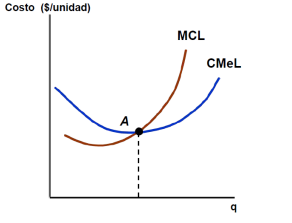
\includegraphics[H]{Captura de pantalla 2026-05-20 092739.png}

%------------------------------------------------------------


%=============================================================
\newpage


%------------------------------------------------------------
\subsection*{Ejercicio 1}

Una empresa en competencia perfecta en el corto plazo tiene una curva de costo total:
\[
CT = 500 + q^3 - 20q^2 + 110q
\]

\subsubsection*{(a) (10 pts) Calcule el precio de cierre de la firma en el corto plazo.}

El costo variable es $CV = q^3 - 20q^2 + 110q$, por lo que el costo variable medio es:
\[
CMeV = \frac{CV}{q} = q^2 - 20q + 110
\]

Minimizamos el $CMeV$ derivando e igualando a cero:
\[
\frac{d(CMeV)}{dq} = 2q - 20 = 0 \implies q = 10
\]

El precio de cierre es el $CMeV$ evaluado en $q = 10$:
\[
CMeV(10) = 10^2 - 20(10) + 110 = 100 - 200 + 110 = \boxed{10}
\]

\subsubsection*{(b) (5 pts) Calcule los beneficios en ese punto e indique si son normales, subnormales o sobrenormales.}

\[
IT = p \cdot q = 10 \times 10 = 100
\]
\[
CT(10) = 500 + 10^3 - 20(10^2) + 110(10) = 500 + 1000 - 2000 + 1100 = 600
\]
\[
\pi = IT - CT = 100 - 600 = -500
\]

La empresa tiene \textbf{beneficios subnormales} (pérdidas económicas).

\subsubsection*{(c) (5 pts) Formule la curva de oferta (u oferta inversa) de la firma.}

El costo marginal es:
\[
CMg = \frac{dCT}{dq} = 3q^2 - 40q + 110
\]

La curva de oferta de la firma es una función por tramos:
\[
q(P) = \begin{cases} 0 & \text{si } P < 10 \\ P = 3q^2 - 40q + 110 & \text{si } P \geq 10 \end{cases}
\]

%------------------------------------------------------------
\subsection*{Ejercicio 2}

El maíz es producido en condiciones de competencia perfecta. Cada productor individual tiene una curva de costos medios a largo plazo con forma de U, alcanzando su mínimo en \$4 por tonelada cuando produce 500 toneladas.

\subsubsection*{(a) (12 pts) Determine el precio de equilibrio de largo plazo y las toneladas demandadas en total.}

La curva de demanda del mercado está dada por:
\[
Q_D = 1{,}500{,}000 - 125{,}000\,P
\]

En competencia perfecta a largo plazo, el precio de equilibrio es igual al costo medio mínimo:
\[
P^* = 4 \text{ dólares por tonelada}
\]

Sustituyendo en la ecuación de demanda:
\[
Q_D = 1{,}500{,}000 - 125{,}000(4) = 1{,}500{,}000 - 500{,}000 = \boxed{1{,}000{,}000 \text{ toneladas}}
\]

\subsubsection*{(b) (8 pts) ¿Cuántos productores habrá en el mercado y cuál será la utilidad de cada uno?}

Cada productor produce 500 toneladas al costo medio mínimo, por lo que:
\[
NF = \frac{Q_D}{\text{Producción por productor}} = \frac{1{,}000{,}000}{500} = \boxed{2{,}000 \text{ productores}}
\]

En equilibrio de largo plazo, la utilidad económica es cero, ya que $P = CMe = 4$:
\[
IT = 4 \times 500 = 2{,}000 \text{ dólares}
\qquad
CT = 4 \times 500 = 2{,}000 \text{ dólares}
\]
\[
\pi = 2{,}000 - 2{,}000 = \boxed{0 \text{ dólares por productor}}
\]

\end{document}